\section{Analysis and Ablations}
\label{sec:ablations}

We further ask the following Research Questions (RQs) to investigate in a finer granularity how to enhance performance optimally.




\subsection{Data Combination Analysis}

\paragraph{\textbf{RQ1: How important is it to have real C4 data?}}

\begin{figure}[t]
\centering
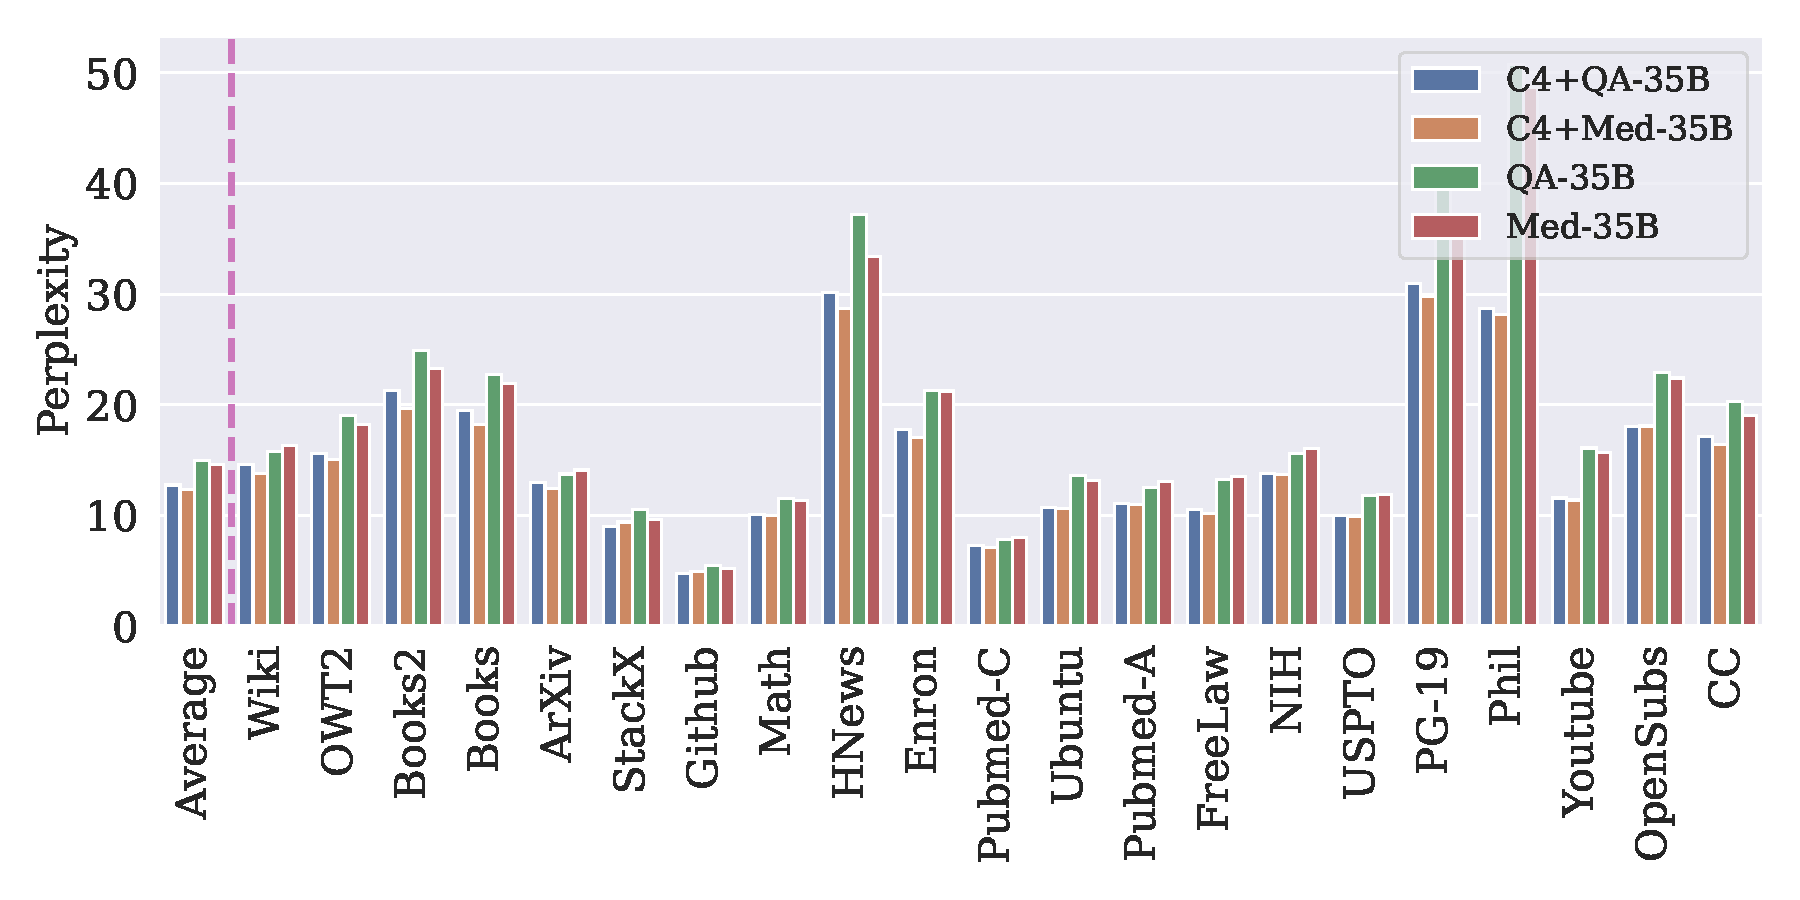
\includegraphics[width=\linewidth]{figures/all_pile_synth_vs_real_style_1.3B_150k.pdf}

\caption{\textbf{Importance of Real Data:} Comparing perplexity on the Pile when pre-training on C4 with synthetic data vs. synthetic data only.  Models are 1.3B parameters trained for a total of 150B tokens on a real data subset containing 35 Billion tokens of the C4.}
\label{fig:syn_comp}
\end{figure}

\begin{table*}[t]
    \centering
    \scalebox{0.8}{
    \begin{tabular}{lcccccccc>{\columncolor{LightCyan}}c}
        \toprule
        Dataset (Real Tok.) & ARC-E & BoolQ & Wino. & PIQA & HellaSwag & TruthfulQA & OBQA & LogiQA & Avg \\
        \midrule
        Med+C4-35B  & 59.8  &  57.0  &  55.7  &  74.6  &  44.5  &  36.5  &  23.8  &  21.5  &  46.7\\
        QA+C4-35B &  62.2  &  63.3  &  55.7  &  74.8  &  44.6  &  41.4  &  22.4  &  23.2  &  48.4\\
        Med-35B &  56.6  &  59.5  &  53.4  &  74.0  &  41.9  &  36.3  &  22.2  &  22.7  &  45.8\\
        QA-35B &  61.7  &  62.0  &  53.9  &  75.2  &  43.4  &  43.0  &  22.8  &  23.4  &  48.2\\
        \bottomrule
    \end{tabular}}
    \caption{\textbf{Importance of Real Data:} Evaluation of $\sim1.3$B parameter LLMs trained for 150B tokens on General Understanding Tasks. Results show that adding real data helps improve model performance when pre-training on `Medium' or `Wikipedia-style' paraphrases. 
    }
    \label{tab:general_understanding_150B_real_data}
\end{table*}

\begin{table*}[t]
    \centering
    \scalebox{0.8}{
    \begin{tabular}{lccccc>{\columncolor{LightCyan}}c}
        \toprule
        Dataset (Real Tok.) & ARC-C & SciQ & PubMedQA & MathQA & MMLU & Avg \\
        \midrule
       Med+C4-35B & 27.2  &  82.2  &  46.2  &  23.1  &  25.2  &  40.8\\
        QA+C4-35B & 29.0  &  85.1  &  62.2  &  22.5  &  26.1  &  45.0\\
        Med-35B & 27.0  &  80.0  &  59.4  &  22.5  &  24.7  &  42.7\\
        QA-35B &  27.1  &  85.5  &  59.2  &  22.2  &  25.0  &  43.8\\
        \bottomrule
    \end{tabular}}
    \caption{\textbf{Importance of Real Data:} Evaluation of $\sim1.3$B parameter LLMs on Specialized Knowledge Tasks.
    Results show that adding real data helps improve model performance when pre-training on `Q/A-style' paraphrases. }
    \label{tab:specialized_knowledge_real_data}
\end{table*}





\begin{table*}[t]
    \centering
    \scalebox{0.8}{
    \begin{tabular}{lccccc>{\columncolor{LightCyan}}c}
        \toprule
        Dataset (Real Tok.) & ARC-C & SciQ & PubMedQA & MathQA & MMLU & Avg \\
        \midrule
       Med+C4-35B & 27.2  &  82.2  &  46.2  &  23.1  &  25.2  &  40.8\\
        QA+C4-35B & 29.0  &  85.1  &  62.2  &  22.5  &  26.1  &  45.0\\
        Combined-1:1-35B &  28.2  &  85.9  &  61.2  &  23.2  &  23.9  &  44.5 \\
        Combined-1:2-35B &  29.0  &  85.7  &  57.4  &  23.5  &  23.1  &  43.7\\
        \bottomrule
    \end{tabular}}
    \caption{\textbf{Combining multiple styles:} Evaluation of $\sim1.3$B parameter LLMs trained for 150B tokens on `Specialized Knowledge Tasks'. Results suggest that combining rephrasing styles does not yield performance benefit on zero-shot tasks compared to just Q/A style.}
    \label{tab:specialized_knowledge_combination}
\end{table*}


\begin{table*}[t]
    \centering
    \scalebox{0.8}{
    \begin{tabular}{lcccccccc>{\columncolor{LightCyan}}c}
        \toprule
        Dataset (Real Tok.) & ARC-E & BoolQ & Wino. & PIQA & HellaSwag & TruthfulQA & OBQA & LogiQA & Avg \\
        \midrule
        Med+C4-35B &  59.8  &  57.0  &  55.7  &  74.6  &  44.5  &  36.5  &  23.8  &  21.5  &  46.7\\
        QA+C4-35B &  62.2  &  63.3  &  55.7  &  74.8  &  44.6  &  41.4  &  22.4  &  23.2  &  48.4\\
        Combined-1:1-35B &  60.6  &  60.2  &  57.7  &  73.8  &  43.7  &  40.2  &  22.0  &  22.1  &  47.5\\
        Combined-1:2-35B &  61.4  &  62.0  &  57.0  &  74.8  &  44.6  &  39.5  &  23.0  &  21.3  &  48.0 \\
        \bottomrule
    \end{tabular}}
    \caption{\textbf{Combining multiple styles:} Evaluation of $\sim1.3$B parameter LLMs trained for 150B tokens on General Understanding Tasks. 
    Results suggest that combining rephrasing styles does not yield performance benefit on zero-shot tasks compared to just Q/A style.}
    \label{tab:general_understanding_combination}
\end{table*}

\begin{figure}[t]
\centering
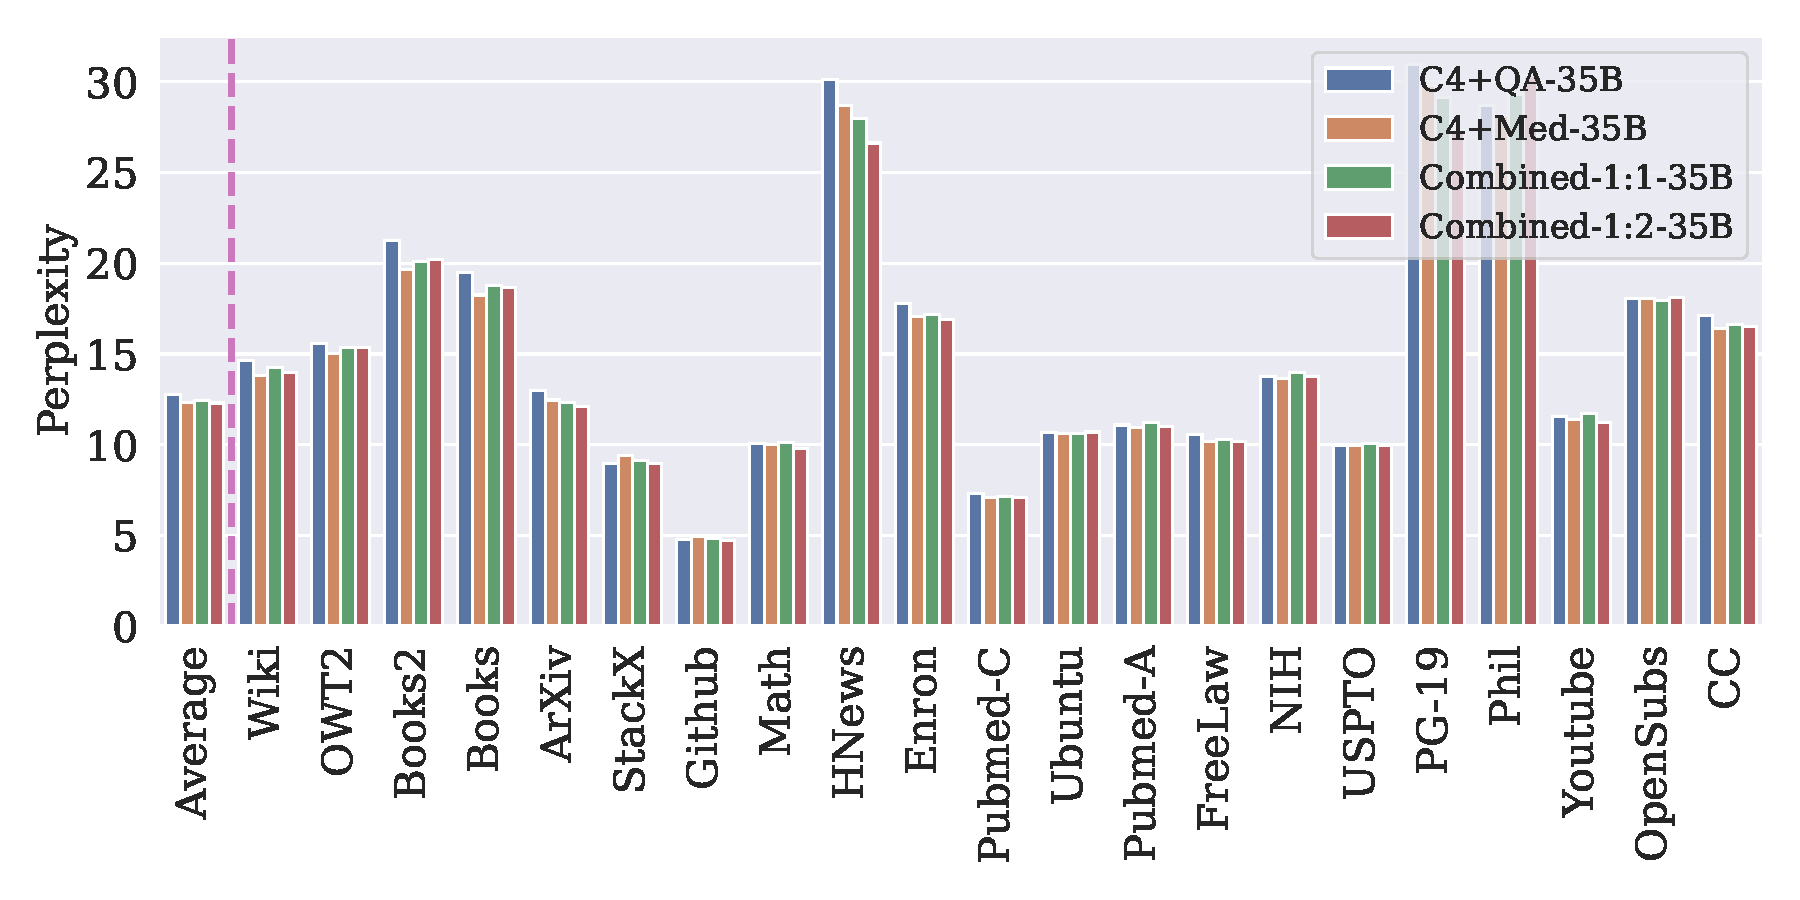
\includegraphics[width=\linewidth]{figures/all_pile_combined_style_1.3B_150k.pdf}
\caption{\textbf{Combining multiple styles:} Perplexity across all domains of the Pile comparing combining multiple styles of synthetic data.  Models are 1.3B parameters trained for a total of 150B tokens. We see small perplexity improvements from combining multiple styles.}
\label{fig:combined_styles}
\end{figure}
Our findings in Tables~\ref{tab:general_understanding}--\ref{tab:specialized_knowledge}indicate that synthetic data using the QA prompt are sufficient for strong performance on QA tasks.  However, when evaluated on Pile perplexity, we observe significant degradation in perplexity across many sub-domains in Figure~\ref{fig:syn_comp}.  This is likely because synthetic data is very clean containing few special characters and being highly structured.  In contrast several sub-domains of the Pile such as OWT, and Hackernews have such special tokens.  On domains such as Philpapers and Gutenberg, we observe that dropping real C4 text from the pre-training data, and training on synthetic documents alone drops performance significantly (increase in perplexity). This is once again attributed to the fact that synthetic data does not contain certain `tags' and `styles' that are prevalent in real data scrapes, and emphasized how \ours~is a better strategy than pre-training on synthetic data alone.
In terms of performance on zero-shot tasks, we once again note that the presence of real data helps improve zero-shot performance in Tables~\ref{tab:general_understanding_150B_real_data},\ref{tab:specialized_knowledge_real_data}.
Since zero-shot tasks contain well-written Q/A pairs, this effect is not as evident as that for perplexities on real data.





 



\paragraph{\textbf{RQ2: Does a combination of multiple synthetic datasets improve performance?}}
We measure the impact of combining multiple synthetic styles with C4 for training.  We consider two variants: combining in a 1:1 ratio meaning that there are two copies of C4 to match two synthetic styles (medium and QA), and 1:2 ratio which combines only one instance of the C4 dataset.  For zero-shot QA tasks, our finding in Table~\ref{tab:specialized_knowledge_combination}-\ref{tab:general_understanding_combination}
 indicate lower performance than combining only QA and C4 data. Evaluations over the Pile are shown in Figure~\ref{fig:combined_styles}.  We notice that both the `Q/A' and `Wikipedia' paraphrases help improve performance on certain domains. For example, `Stackexchange', that has lots of question-answers benefits from the presence of synthetic data in Q/A style. Overall, we note that there is a small improvement on the average perplexity on the Pile by combining multiple styles.


\subsection{Method Ablations}

\paragraph{\textbf{RQ3: How important is to have a high-quality re-phraser?}}

\begin{figure}[t]
\centering
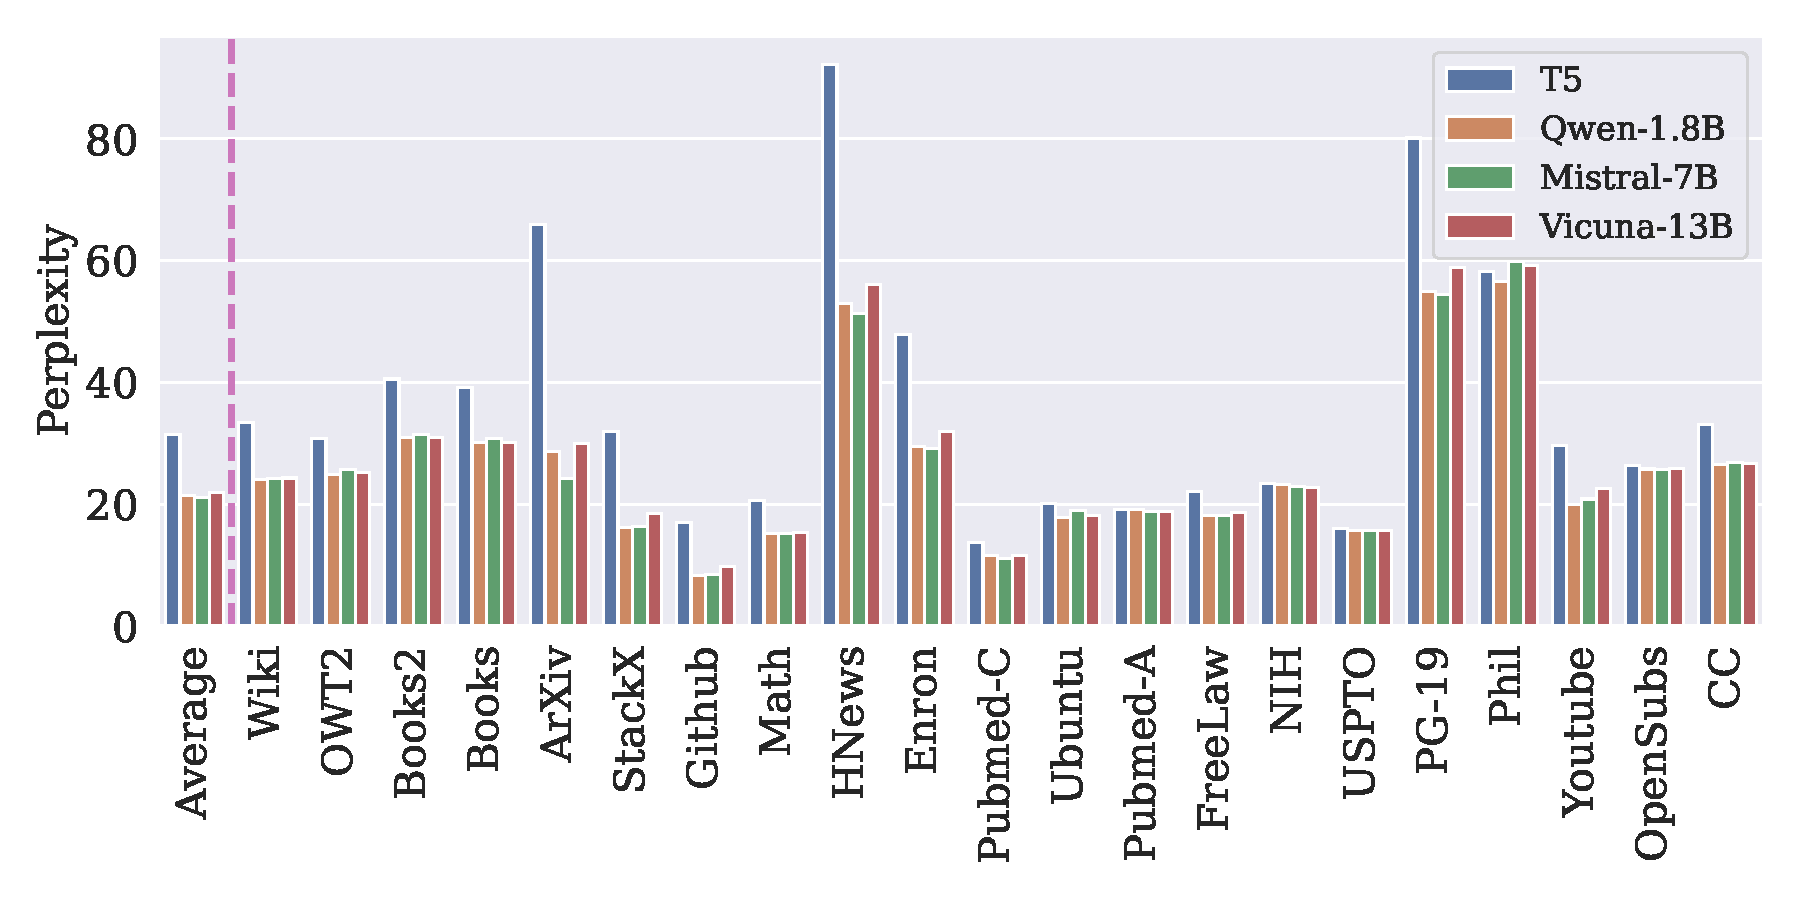
\includegraphics[width=\linewidth]{figures/all_pile_archs_345M_30k.pdf}
\caption{\textbf{Importance of High Quality Paraphraser:} Perplexity across all the Pile domains for \ours~on data generated by different LLMs.
Results show that even small models like Qwen-1.8B can generate paraphrases of high quality. Though, a low quality rephraser like our fine-tuned T5-base model leads to significantly worse language modeling.
}
\label{fig:model_rephraser}
\end{figure}

\begin{figure}[t]
\centering
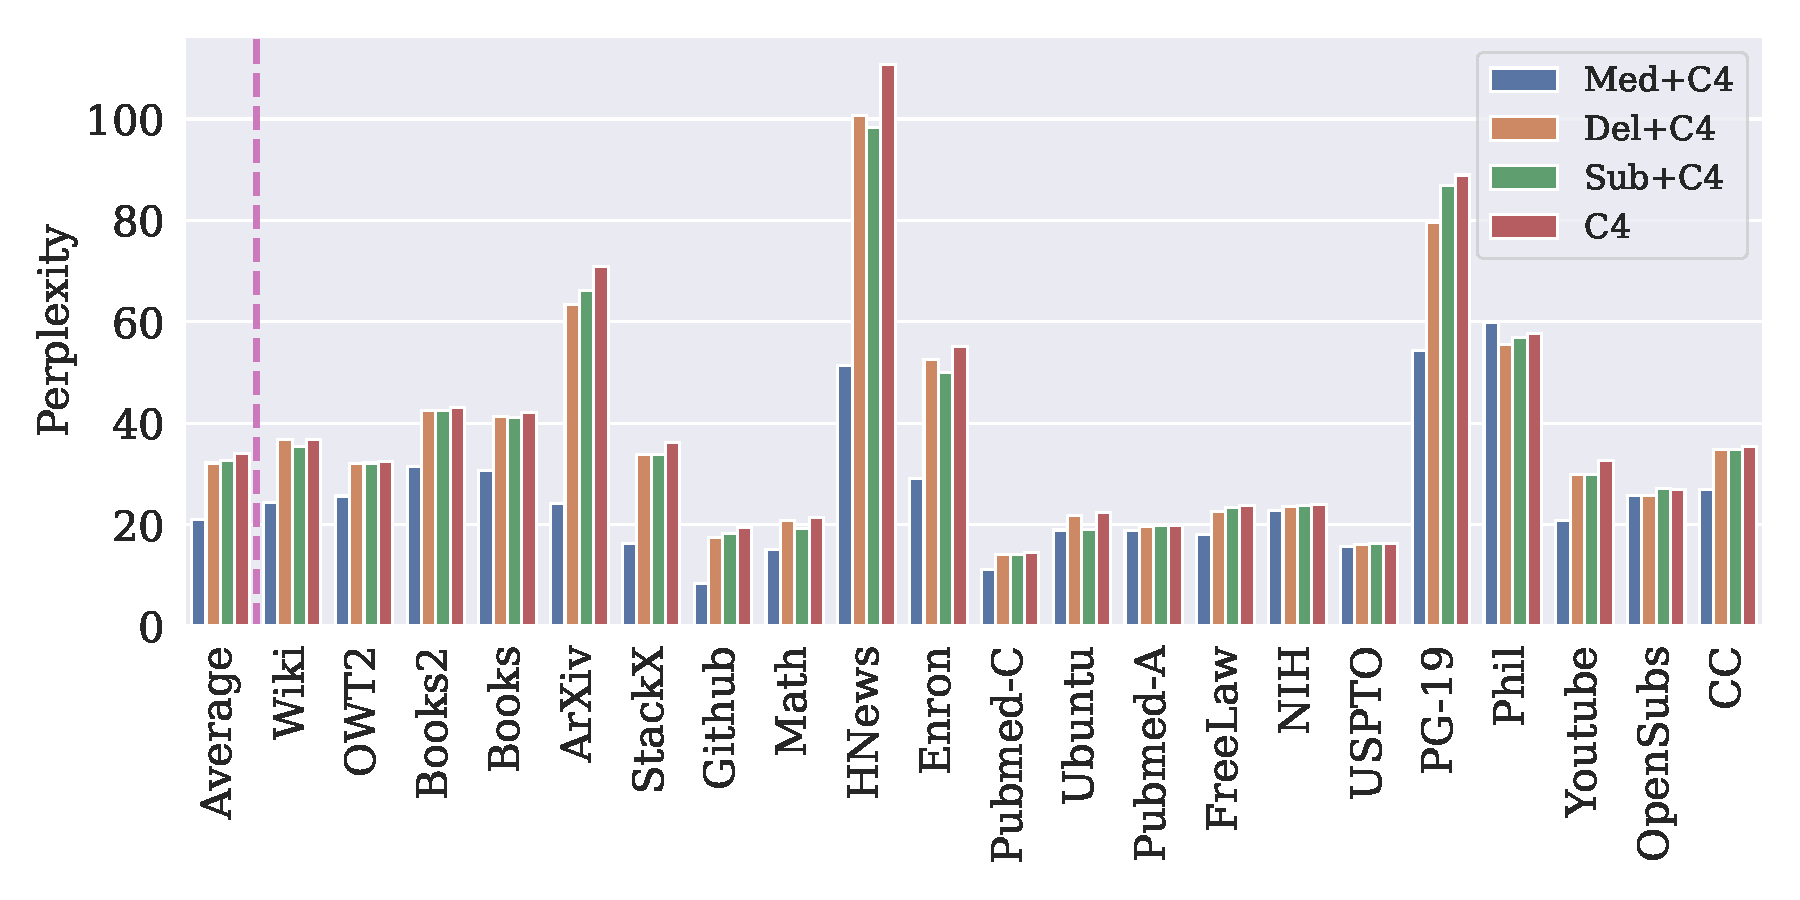
\includegraphics[width=\linewidth]{figures/all_pile_augs_350M_30k.pdf}
\caption{\textbf{Is re-phrasing same as any augmentation?} We compare perplexity on the Pile for different augmemntation strategies.  350M parameter models are trained for a total of 15B tokens. \ours~(Medium + C4) performs significantly better than traditional augmentations.}
\label{fig:augs}
\end{figure}


To answer this,
we use data from four distinct re-phrasing models (T5-base~\citep{raffel2020exploring}, Qwen-1.8B-chat~\citep{qwen}, Mistral-7B-chat~\citep{jiang2023mistral}, and Vicuna-13B-chat-v1.3~\citep{vicuna2023}) and train a 345M model for 30B tokens.  We generate data from all models using the same prompt.  In case of the T5-base model, we finetune the model for 1 epoch on re-phrase pairs from the Vicuna-13b-chat  model. 
We find that pre-training on data generated by smaller re-phrase models like Qwen-1.8B and Mistral-7B achieve lower perplexity than 
Vicuna~13B
(Figure~\ref{fig:model_rephraser}).  
At the same time, our fine-tuned T5-base model performs significantly worse than the rest.
Even then, all rephrase models reduce perplexity over only real C4 data. 
It remains an open question to test the limits of how small can we train a paraphrase model that can generate high quality synthetic data to further scale the applicability of \ours.

\paragraph{\textbf{RQ4: Does synthetic data improve over augmentations?}}
Are the gains observed by pre-training on synthetic data the same as pre-training with augmentations? In order to test this, 
we consider two popular text augmentation baselines---synonym replacement and random deletion using the NL-Augmenter library~\citep{dhole2021nlaugmenter}.
We pre-train a 350M parameter model for 15B tokens in order to conduct this set of experiments. The total pool size is only about 1.5B tokens, meaning that the model would have to repeat data around 10 times during the pre-training phase, unless augmented over.
As seen in the perplexity analysis in Figure~\ref{fig:augs}, the models trained on augmented data perform significantly worse than those trained on combinations of real and synthetic data. This suggests that synthetic data enhances the learning process, and is not merely another form of augmentation.





\paragraph{\textbf{RQ5: How does the style of synthetic data impact performance on specialized domains?}}

 \begin{figure}[t]
\centering
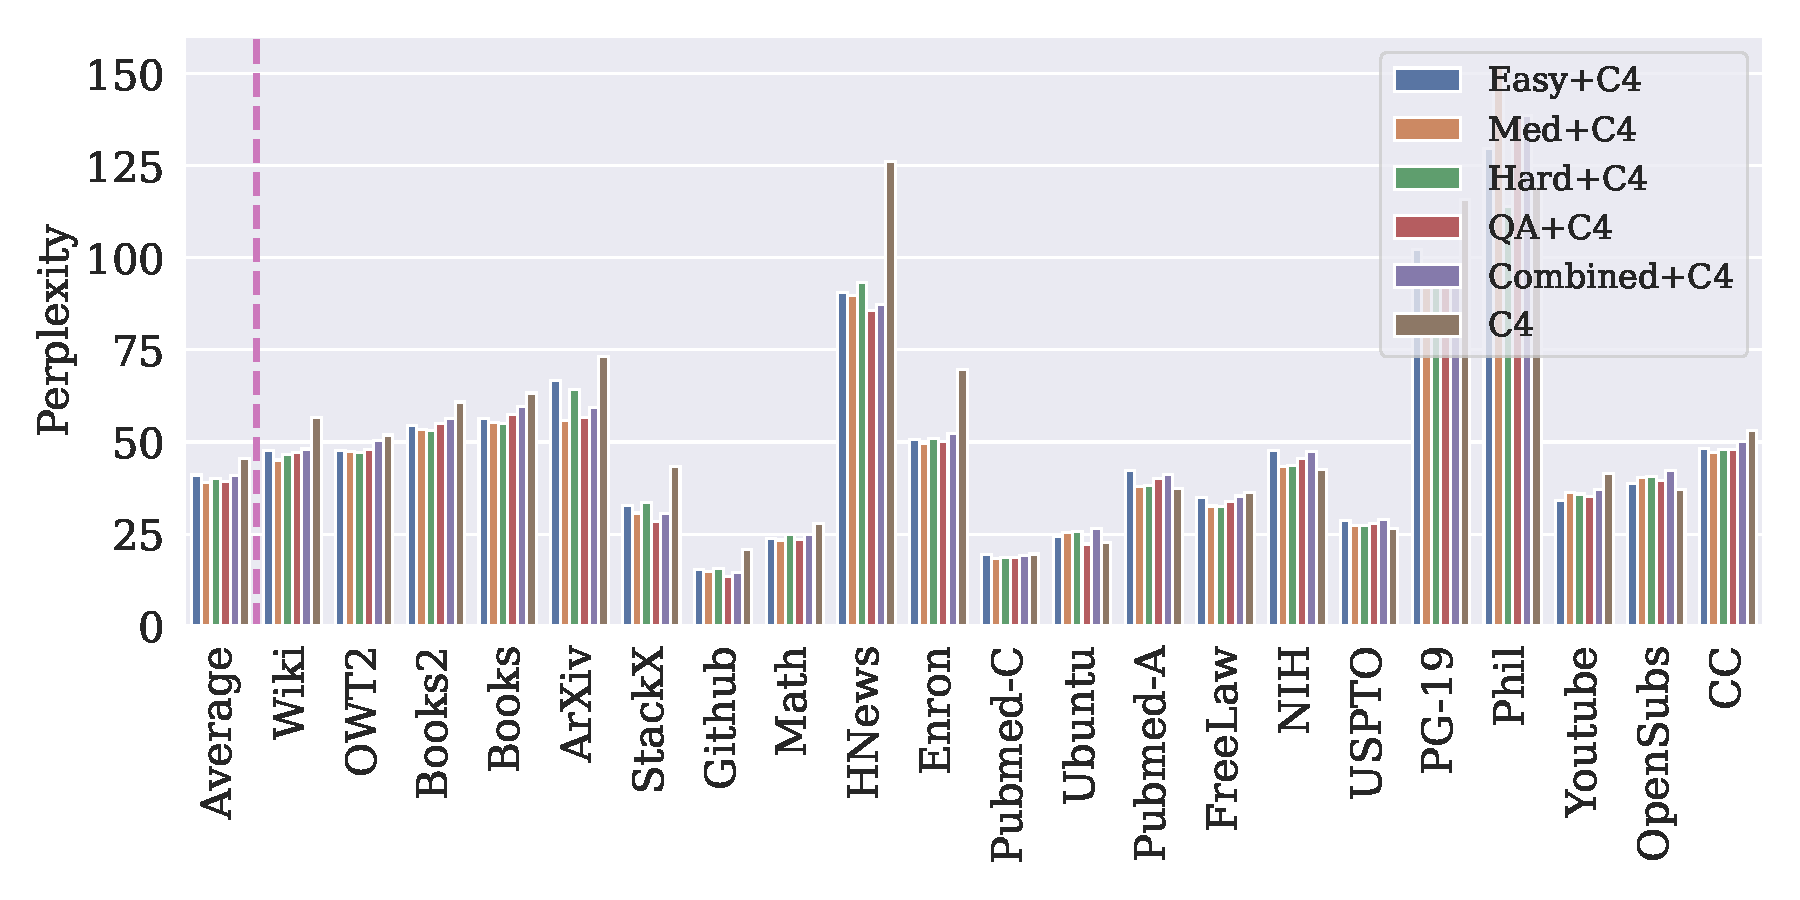
\includegraphics[width=\linewidth]{figures/all_pile_styles_128M_6k.pdf}
\caption{\textbf{Impact of style of synthetic rephrases:} Perplexity across all domains of the Pile comparing different styles of synthetic data.  We train 128M parameter models for 3B tokens.}
\label{fig:styles}
\end{figure}
We compare the performance of various models trained on different styles of synthetic data.  In particular, we generate four styles of synthetic data (easy, medium, hard, and Q/A) and evaluate the performance of training on combinations of each style across Pile subsets. The prompts to generate these synthetic data styles are outlined in Appendix~\ref{app:prompt_styles}. Results corresponding to generations from a Vicuna-v1.3 model, and for a 128M model trained for 3B tokens are summarized in Figure~\ref{fig:styles}.
We see  that training with combinations of real C4 and synthetic data matching the style of the domain at evaluation improves performance.  However, we find that no single synthetic data style performs the best across all domains, resulting in similar performance across training with combinations of real C4 data and each synthetic style variant.  While knowing the best synthetic style to pre-train an LLM is impractical, an oracle that selects the best synthetic style across all domains will improve perplexity by 16\%---indicating the importance of training with diverse data styles for LLM generalization, even when the underlying knowledge stays the same.  


\paragraph{\textbf{RQ6: Is there data leakage from the rephrase model to the trained model?}}

We investigate whether our synthetic data maintains similar semantic meaning while being stylistically different from the original C4 data and matching the style of different PILE domains.  We start by comparing pairs of examples of synthetic and real data to confirm the performance gain is not attributed to knowledge leakage from the rephrase models.  We take a subset of the first 1000 samples from each of the datasets. 

We show the cosine similarity of the sentence embeddings from a pre-trained BERT model trained with SimCSE objective \citep{gao2021simcse} for medium and qa prompts in  Figure~\ref{fig:cosine_sim_style}(a)  and (b).  When computing similarity, we remove outliers. Figures with distributions use a gaussian Kernel Density Estimator (KDE) to construct distributions for statistics from 1000 values. The cosine similarity of real-synthetic pairs is higher than several baselines including  two random real samples from C4, a continuation baseline which computes cosine between the first half of a sample and the full sample, and cosine similarity between the first half and second half of the same sample. High similarity indicates that the re-phrases maintain similar meaning to their real counterparts without adding information. 




\begin{figure*}
  \centering
  \begin{subfigure}{0.45\linewidth}
    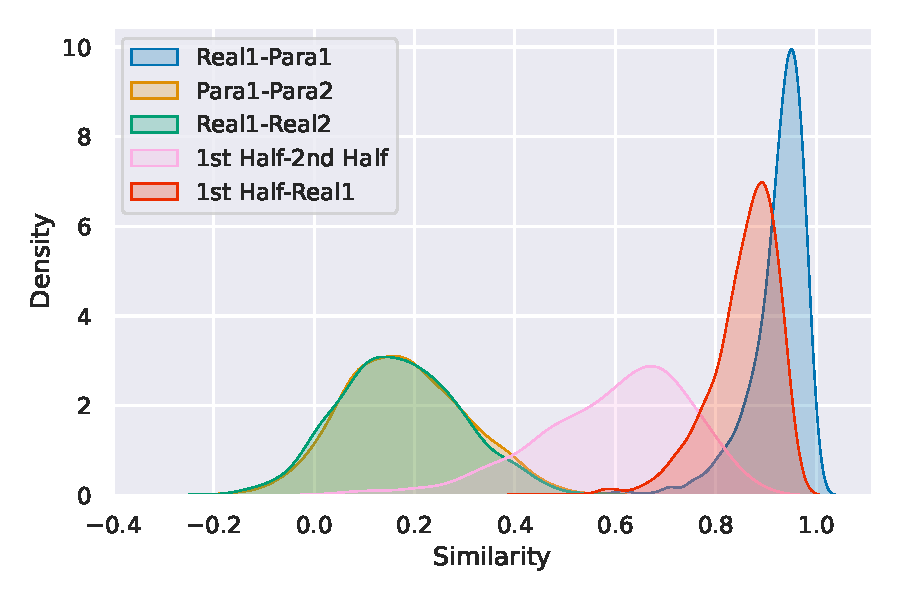
\includegraphics[width=\columnwidth]{figures/medium_cosine_sim_comparison.pdf}
    \caption{Cosine similarity Medium synthetic data}
  \end{subfigure}
  \hfill
  \begin{subfigure}{0.45\linewidth}
    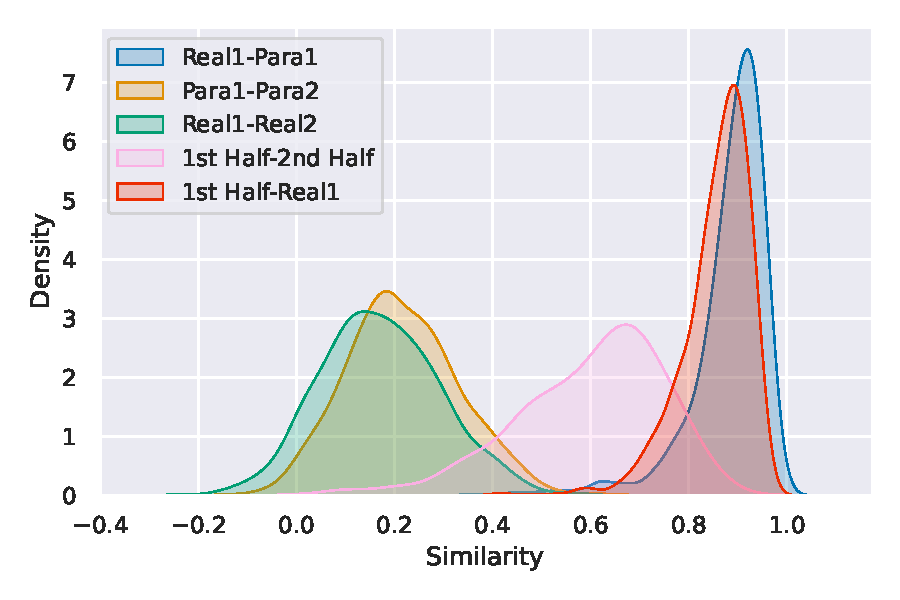
\includegraphics[width=\columnwidth]{figures/qa_cosine_sim_comparison.pdf}
    \caption{Cosine similarity QA synthetic data}
  \end{subfigure}
  \hfill
  \caption{Comparison between synthetic and real data from the C4 corpus showing that synthetic data maintains semantic meaning compared with the real C4 data and primarily changes style for (a) medium rephrases of C4, and (b) QA rephrases of C4.} %
  \label{fig:cosine_sim_style}
\end{figure*}















